\documentclass[12pt]{report}
\usepackage{amsmath}
\usepackage{graphicx}
\usepackage{hyperref}
\usepackage[utf8]{inputenc}
\usepackage{listings}

\title{CS3031 Advanced Telecommunications \\ Project II}
\author{Séamus Woods \\ 15317173}
\date{05/04/2019}

\begin{document}
\maketitle
\newpage


\section{Specification}
The objective of the excercise is to develop a secure cloud storage application for Google Drive. For example my application will secure all files that are uploaded to the cloud, such that only people that are part of my 'Secure Cloud Storage Group' will be able to decrypt my uploaded files. To all other users the files will be encrypted. I was required to design and implement a suitable key management system for my application that will allow me to share files securely, and add or remove users from my group. 
\newline

\section{Implementation}
The easiest way to explain my design and implementation is just by talking through the execution of the code below. I have successfully managed to implement all features listed above. 
\newline
For a brief overview, there are three main files for this program. $drive.py$, $client.py$ and $server.py$.
\newline
\newline
$drive.py$ is the admin side of the application, here the admin can encrypt/decrypt all the files in the drive, add/remove users to the group and see what files are in the drive.
\newline
\newline
$client.py$ is intended to be that part of the application that the client uses. Here they can login, see what files are in the drive, view the contents of files and upload/delete files from the drive.
\newline
\newline
$server.py$ is a flask server, which listens for client.py to send it a username, and will return the encrypted version of the symmetric key for that user to the client, where it can then be decrypted.
\newline
\newline
How does the encryption work? After you choose which folder of your drive you wish to be encrypted, you choose to option to encrypt all files in $drive.py$, this will generate a symmetric key and use that to encrypt all files in the folder. If a user is added to the group, they're given an assymetric key. If that user requests to view the contents of a file, we encrypt the symmetric key with their public key, give that to them using $server.py$ and then they can decrypt that using their private key, verifying that they're part of the group. If a user is removed, we delete their asymmetric key, decrypt all the files in the folder with the symmetric key, generate a new symmetric key and re-encrypt all the files in the folder of the drive.
\newline
\newline
Some screenshots and code can be seen below.
\newline
Server side after selecting to view users..
\begin{center}
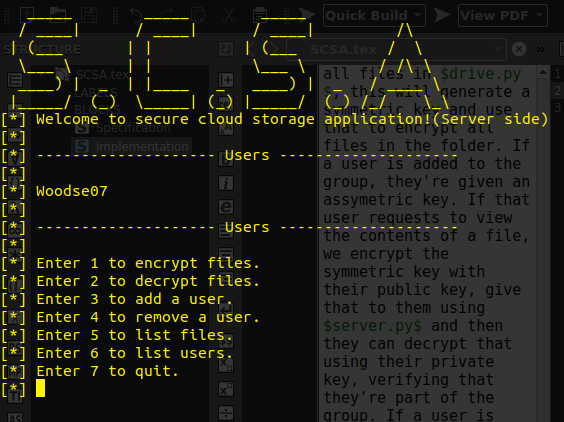
\includegraphics[scale=0.5]{server1.png}
\end{center}
Server side after adding user 'John'
\begin{center}
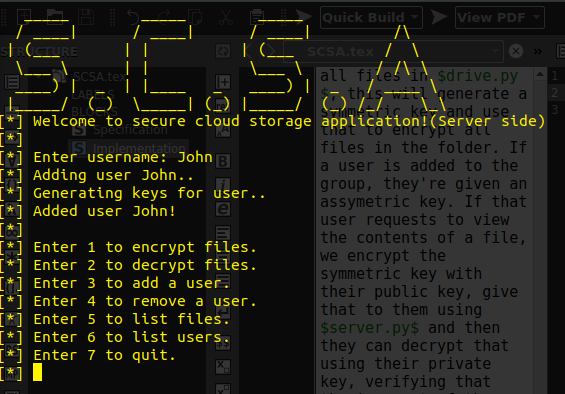
\includegraphics[scale=0.5]{server2.png}
\end{center}
Client side after logging in as 'John'
\begin{center}
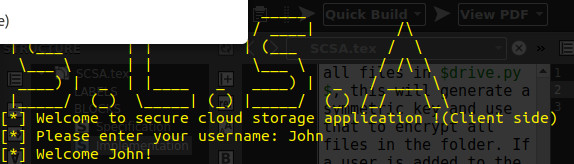
\includegraphics[scale=0.5]{client1.png}
\end{center}
Client side after requesting to view 'secret1.txt'
\begin{center}
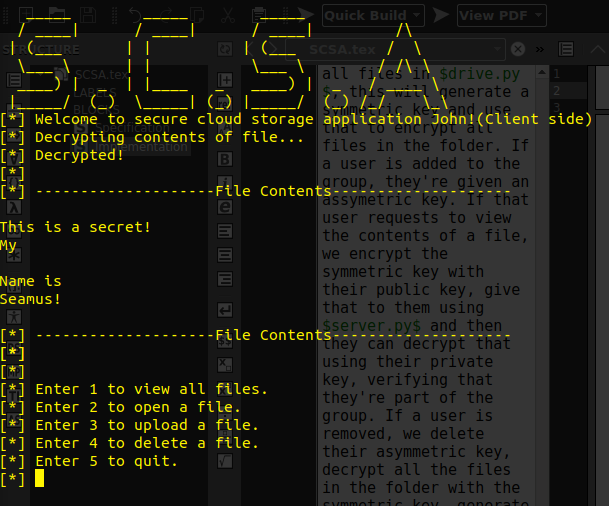
\includegraphics[scale=0.5]{client2.png}
\end{center}

\section{Drive.py}
\lstset{%
  language=Python,
  basicstyle=\footnotesize,
  showstringspaces=false,
  numbers=left,
  breakatwhitespace=false,
  breaklines=true,
  breakatwhitespace=true,
}
\lstinputlisting[language=Python]
{drive.py}

\section{Client.py}
\lstset{%
  language=Python,
  basicstyle=\footnotesize,
  showstringspaces=false,
  numbers=left,
  breakatwhitespace=false,
  breaklines=true,
  breakatwhitespace=true,
}
\lstinputlisting[language=Python]
{client.py}

\section{Server.py}
\lstset{%
  language=Python,
  basicstyle=\footnotesize,
  showstringspaces=false,
  numbers=left,
  breakatwhitespace=false,
  breaklines=true,
  breakatwhitespace=true,
}
\lstinputlisting[language=Python]
{server.py}


\end{document}
